\documentclass[12pt]{article}
\usepackage[utf8]{inputenc}
\usepackage{amsmath, amssymb, graphicx, hyperref, enumitem}
\usepackage[a4paper, margin=1in]{geometry}

\title{Terminal-Based Spreadsheet Application: Design and Architecture Report}
\author{Lucky Ahirwar \\
        2022CS52049 \\
        \and Swapnil \\
        2022ME21540 \\
        \and Namrata Sinha \\
        2021ME10995 }
\date{\today}

\begin{document}

\maketitle

\section{Software Architecture}

The terminal-based spreadsheet application is structured using a modular architecture designed for efficiency, clarity, and scalability. The architecture is composed of the following primary modules:

\subsection{Parser and Evaluator}
\textbf{Parser:} Interprets user input, extracts commands and formulae, and detects syntactic errors.\\
\textbf{Evaluator:} Processes the parsed commands, manages dependencies, and updates the spreadsheet. It ensures:

\subsection{Data Storage Module}
The spreadsheet uses a \texttt{HashMap}-based design for efficient and scalable storage of cell data. This replaces the earlier deque-based column-segment model with a flat key-value approach. The key is a 32-bit integer uniquely encoding a cell's position (e.g., using \texttt{row * 1000 + col}), and the value is a \texttt{Cell} struct holding data and metadata.

\begin{itemize}
  \item \textbf{Database Structure:}
  \begin{itemize}
    \item Uses \texttt{HashMap<u32, Cell>} to store cell data efficiently.
    \item \texttt{range\_deps: DepStore}: Manages dependencies for range-based formulas (e.g., \texttt{SUM(A1:A5)}). Uses DepStore, which is wrapper around R-Tree.
    \item \texttt{point\_deps: HashMap<u32, Vec<u32>>}: Tracks non-range dependencies between individual cells.
  \end{itemize}

  \item \textbf{Cell Metadata:} Each \texttt{Cell} contains:
  \begin{itemize}
    \item \texttt{data: CellData}: Holds either integer or floating-point data.
    \item \texttt{error: bool}: Indicates if the cell has an error.
    \item \texttt{dependencies: Option<DependencyData>}: Describes the operation and involved values or cell references.
  \end{itemize}

  \item \textbf{Dependency Representation:}
  \begin{itemize}
    \item \texttt{DependencyData}: Encodes formulas using an operator and two operands (\texttt{pre}, \texttt{post}), both wrapped in the \texttt{DependencyNums} enum, which can store integers, floats, or encoded cell references.
    \item \texttt{DependencyObject}: Associates a dependency with its target cell for efficient graph updates.
  \end{itemize}
\end{itemize}

\subsection{Dependency Graph}
Each cell maintains a field \texttt{dependencies: Option<DependencyData>} which encodes dependency data. Dependencies are also stored inside the database struct. Inside database struct, we store range dependencies and non-range dependencies differently.

\subsection{User Interface (UI)}
C lab port UI terminal I/O, accepting user commands and rendering results. It displays time taken for evaluation, any parsing/evaluation errors, the visible portion of the spreadsheet.

Rust lab extension uses Ratatui to render the grid, status bar, menus, and ASCII-based charts. Also reflects errors. crossterm backend captures and processes key events directing them appropriately based on the current mode (e.g., View, Insert, Visual). Insert mode commands are handled partially by parser and evaluator.

\subsection{Integration Workflow}
The user interaction and processing flow is as follows:
\begin{enumerate}
  \item User inputs a command (e.g., formula or value).
  \item The Parser processes and validates the input.
  \item The Evaluator updates the dependency graph, performs computations, and updates the database.
  \item The UI module reflects these changes on-screen.
\end{enumerate}


\section{Data Structures Used}
To ensure efficient performance, scalability, and responsiveness, the following data structures were employed:

\begin{itemize}
    \item \textbf{HashMap:}
    \begin{itemize}
        \item Used in the \texttt{Database} module to store cell data.
        \item Keys are 32-bit integers uniquely encoding the row-column position.
        \item Values are \texttt{Cell} structs that hold the actual content and metadata.
    \end{itemize}

    \item \textbf{RTree:}
    \begin{itemize}
        \item Used in the \texttt{DepStore} module for efficient range dependency tracking.
        \item Dependencies across ranges (e.g., \texttt{SUM(A1:A10)}) are represented using \texttt{DependencyObject} structs and stored in an \texttt{RTree}.
        \item Supports fast spatial queries using bounding boxes (AABB) to determine if a cell lies within any dependent range.
        \item Enables quick lookups of dependencies involving ranges.
    \end{itemize}


    \item \textbf{Graph (Dependency Graph):}
    \begin{itemize}
        \item Used to track and manage dependencies between cells, both direct and range-based.
        \item Supports cycle detection, topological sorting, and efficient update propagation.
    \end{itemize}

    \item \textbf{Custom Enums and Structs:}
    \begin{itemize}
        \item \texttt{CellData} enum stores either integer or floating-point data.
        \item \texttt{DependencyNums} enum generalizes operands in dependencies as integers, floats, or encoded cell references.
        \item \texttt{DependencyData} represents a formula as an operation and two operands (\texttt{pre} and \texttt{post}).
        \item \texttt{DependencyObject} wraps the dependency along with its target cell, used in the RTree.
    \end{itemize}
\end{itemize}

\section{Extensions}
\begin{figure}[ht]
    \centering
    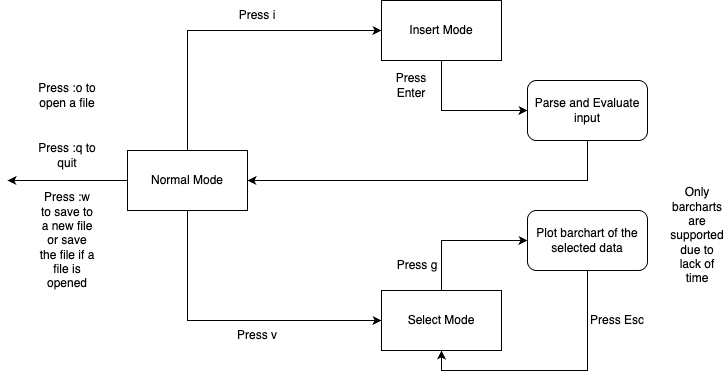
\includegraphics[width=0.8\textwidth]{report/rust_flow.png}
    \caption{Program flow of the extension mode}
    \label{fig:high_level_design}
\end{figure}

\section{Why Proposed Extensions Could Not Be Implemented}

\begin{itemize}
\item \textbf{Graphical Extensions}: The ASCII graph/chart module was partially implemented, but dynamic chart rendering over large datasets was not stable due to limitations in terminal rendering and Ratatui's layout flexibility.
\item \textbf{Machine Learning Metrics}: Lack of time and complexity in implementing robust ML evaluation functions with validation checks delayed this feature.
\item \textbf{Undo/Redo History}: Implementing a full undo/redo stack across different spreadsheet states required deeper redesign of the command pattern and serialization of operations.
\end{itemize}

\section{Could We Implement Extra Extensions Over and Above the Proposal?}

\begin{itemize}
\item \textbf{Real-time Collaboration}: A lightweight server-client model using TCP sockets was considered to allow multiple users to edit collaboratively.
\item \textbf{Plugin System}: Possibility of enabling user-defined Rust functions or external script hooks.
\item \textbf{Cell Styling}: Color-coded cells or bold/italic attributes using extended Unicode and Ratatui styling.
\end{itemize}

\section{Interfaces Between Software Modules}

\begin{itemize}
\item UI Renderer communicates with AppState to get cell contents and mode status.
\item Input Handler dispatches parsed commands to the Core Engine.
\item Core Engine signals UI to re-render after mutations.
\item File IO modules encode/decode Grid and metadata via a serialization interface.
\end{itemize}

\section{Approaches for Encapsulation}

\begin{itemize}
\item Core logic is kept in \texttt{src} module. Extensions are defined separately in \texttt{extensions} module. Extensions work independent of the main logic implementation, and use API exposed by the core functions.
\item UI components are in \texttt{ui} module with dedicated structs for widgets.
\item Every module is accessed through their public functions, and implementation details are hidden. This makes it possible to improve parts of the code, without needing to change other parts of the code.
\end{itemize}

\section{Justification for the Design}

\begin{itemize}
\item Modular separation ensures extensibility and testability.
\item Enum-based command dispatching simplifies control flow across modes.
\end{itemize}

\section{Modifications Made to Original Design}

In the initial design of the spreadsheet, each cell stored both its dependencies and dependents as linked lists. While this model was conceptually simple and worked well for small spreadsheets, it suffered from severe performance and memory issues at scale, particularly when dealing with large range-based formulas such as \texttt{SUM(A2:ZZZ999)}.

\subsection{Problems with the Initial Design}
\begin{itemize}
    \item \textbf{Excessive Memory Allocations:} Each dependency and dependent relationship required a separate heap allocation (via \texttt{malloc}). In large spreadsheets, especially with range-based formulas, this led to thousands of tiny allocations, causing memory fragmentation and overhead.
    
    \item \textbf{Complex Update Logic:} Modifying or clearing a formula involved recursively visiting and mutating linked lists spread across many cells, making updates and cycle detection inefficient and error-prone.
\end{itemize}

\subsection{Advantages of the New Centralized Model}
To overcome these limitations, we redesigned the dependency management system using a centralized data structure combining a \texttt{HashMap} and an \texttt{RTree}, with the following benefits:

\begin{itemize}
    \item \textbf{Central Storage:} Dependencies are no longer scattered across individual cells. Instead, they are stored in:
    \begin{itemize}
        \item A \texttt{HashMap<u32, Vec<u32>>} for non-range dependencies.
        \item An \texttt{RTree<DependencyObject>} for range-based dependencies.
    \end{itemize}
    
    \item \textbf{Simplified Cell Structure:} Each \texttt{Cell} now only stores the formula it directly contains (if any), not its dependents. This greatly reduces memory usage per cell and simplifies mutation logic.
    
    \item \textbf{Efficient Range Queries:} The \texttt{RTree} allows us to perform fast spatial queries to check which ranges a given cell is part of. This is particularly useful when updating a cell to propagate changes efficiently.
    
    \item \textbf{Better Performance at Scale:} The new model supports large spreadsheets and formulas with extensive ranges without significant performance degradation.
\end{itemize}

\end{document}